\documentclass[aspectratio=169]{beamer}
\usetheme{Madrid}
\usecolortheme{default}
\usepackage[utf8]{inputenc}
\usepackage[T5]{fontenc}
\usepackage{graphicx}
\usepackage{hyperref}
\usepackage{booktabs}
\usepackage{amsmath}
\usepackage{listings}
\usepackage{xcolor}

\setbeamertemplate{caption}[numbered]
\renewcommand{\figurename}{Hình}
\renewcommand{\thefigure}{12.\arabic{figure}}

% Cấu hình listings cho Python
\definecolor{codegreen}{rgb}{0,0.6,0}
\definecolor{codegray}{rgb}{0.5,0.5,0.5}
\definecolor{codepurple}{rgb}{0.58,0,0.82}
\definecolor{backcolour}{rgb}{0.95,0.95,0.92}

\lstdefinestyle{mystyle}{
    backgroundcolor=\color{backcolour},   
    commentstyle=\color{codegreen},
    keywordstyle=\color{magenta},
    numberstyle=\tiny\color{codegray},
    stringstyle=\color{codepurple},
    basicstyle=\ttfamily\scriptsize,
    breakatwhitespace=false,         
    breaklines=true,                 
    captionpos=b,                    
    keepspaces=true,                 
    numbers=left,                    
    numbersep=5pt,                  
    showspaces=false,                
    showstringspaces=false,
    showtabs=false,                  
    tabsize=2
}
\lstset{style=mystyle}

\title[Chương 12: Object Detection]{Học Sâu (Deep Learning) \\ \vspace{0.5cm} \Large Chương 12: Phát hiện Vật thể \\ (Object Detection)}
\author{Đại học Đông Á}
\date{\today}

\begin{document}

\begin{frame}
    \titlepage
\end{frame}

\begin{frame}{Nội dung chương}
    \tableofcontents
\end{frame}

\section{1. Giới thiệu Bài toán Phát hiện Vật thể}

\begin{frame}{Bài toán Phát hiện Vật thể là gì?}
    \begin{columns}
        \column{0.5\textwidth}
        \begin{itemize}
            \item Không chỉ trả lời câu hỏi "Trong ảnh có gì?" (Classification).
            \item Phải trả lời được "Nó nằm ở đâu?" bằng cách vẽ các \textbf{Hộp giới hạn (Bounding Boxes)}.
            \item \textbf{Ứng dụng thực tế:}
            \begin{itemize}
                \item Xe tự lái: Phát hiện người đi bộ, biển báo.
                \item Bán lẻ: Đếm số lượng sản phẩm trên kệ.
                \item Trích xuất: Cắt vùng biển số xe để đưa vào OCR.
            \end{itemize}
        \end{itemize}
        
        \column{0.5\textwidth}
        \begin{figure}
            \centering
            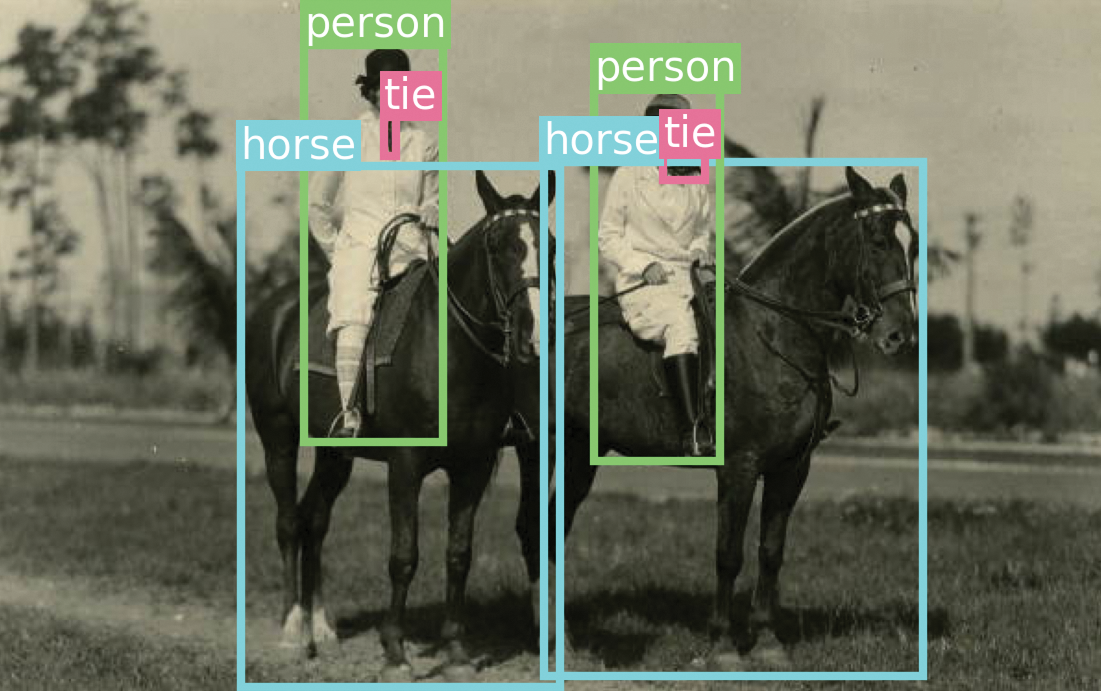
\includegraphics[width=\textwidth,height=0.6\textheight,keepaspectratio]{../../images/ch12/object-detection.7c5cbfd4.png}
            \caption{Vẽ hộp giới hạn và gán nhãn}
        \end{figure}
    \end{columns}
\end{frame}

\begin{frame}{Bộ dữ liệu COCO (Common Objects in Context)}
    \begin{columns}
        \column{0.5\textwidth}
        \begin{itemize}
            \item MS COCO là tiêu chuẩn vàng (Gold Standard) để đánh giá các mô hình Object Detection hiện đại.
            \item Hơn 200,000 hình ảnh được gán nhãn thủ công với 80 danh mục vật thể.
            \item Tính chất đa dạng cao: Nhiều vật thể đan xen, chồng chéo, kích thước từ siêu nhỏ đến khổng lồ trong cùng một khung hình.
        \end{itemize}
        
        \column{0.5\textwidth}
        \begin{figure}
            \centering
            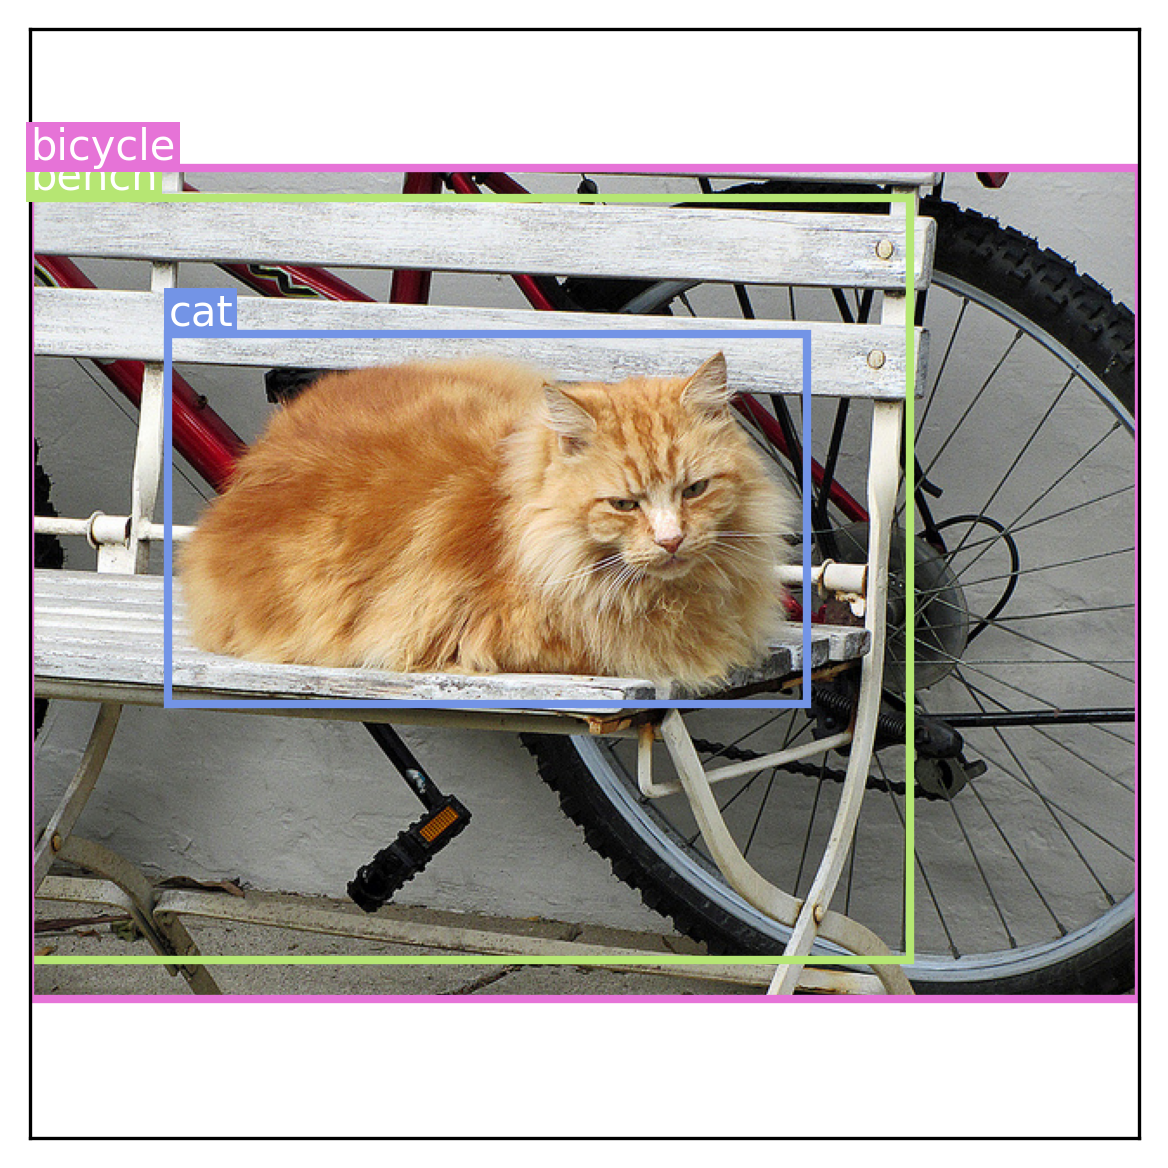
\includegraphics[width=\textwidth,height=0.6\textheight,keepaspectratio]{../../images/ch12/coco-example.c43c39d6.png}
            \caption{Dữ liệu phức tạp trong COCO}
        \end{figure}
    \end{columns}
\end{frame}

\begin{frame}[fragile]{Tải Dữ liệu COCO 2017}
Dữ liệu COCO có dung lượng khổng lồ. Chúng ta tải bộ \texttt{train2017} (khoảng 18GB) và file nhãn (Annotations JSON).

\begin{lstlisting}[language=Python]
import keras
import keras_hub

images_path = keras.utils.get_file(
    "coco",
    "http://images.cocodataset.org/zips/train2017.zip",
    extract=True,
)
annotations_path = keras.utils.get_file(
    "annotations",
    "http://images.cocodataset.org/annotations/annotations_trainval2017.zip",
    extract=True,
)
\end{lstlisting}
\end{frame}

\begin{frame}[fragile]{Xử lý Tọa độ Hộp giới hạn (Bounding Boxes)}
Mỗi hộp trong COCO có tọa độ \texttt{x, y, width, height}. Chúng ta cần chuẩn hóa tọa độ này về tỷ lệ \texttt{[0, 1]} dựa trên kích thước ảnh gốc.

\begin{lstlisting}[language=Python]
import json

with open(f"{annotations_path}/annotations/instances_train2017.json", "r") as f:
    annotations = json.load(f)

# Sorts image metadata by ID
images = {image["id"]: image for image in annotations["images"]}

# Converts bounding box to coordinates on a unit square
def scale_box(box, width, height):
    scale = 1.0 / max(width, height)
    x, y, w, h = [v * scale for v in box]
    x += (height - width) * scale / 2 if height > width else 0
    y += (width - height) * scale / 2 if width > height else 0
    return [x, y, w, h]
\end{lstlisting}
\end{frame}

\begin{frame}[fragile]{Tích hợp Dữ liệu Meta}
Nhóm tất cả các Bounding Boxes và Labels theo từng file hình ảnh.

\begin{lstlisting}[language=Python]
# Aggregates all bounding box annotations by image ID
metadata = {}
for annotation in annotations["annotations"]:
    id = annotation["image_id"]
    if id not in metadata:
        metadata[id] = {"boxes": [], "labels": []}
    image = images[id]
    box = scale_box(annotation["bbox"], image["width"], image["height"])
    metadata[id]["boxes"].append(box)
    metadata[id]["labels"].append(annotation["category_id"])
    metadata[id]["path"] = images_path + "/train2017/" + image["file_name"]

metadata = list(metadata.values())
\end{lstlisting}
Kết quả ta thu được $117,266$ ảnh huấn luyện!
\end{frame}

\begin{frame}[fragile]{Hàm Hỗ trợ Trực quan hóa (Visualization Utilities)}
Để dễ dàng theo dõi Bounding Box trên ảnh, ta viết các hàm phụ trợ dùng \texttt{matplotlib}.

\begin{lstlisting}[language=Python]
import matplotlib.pyplot as plt
from matplotlib.colors import hsv_to_rgb
from matplotlib.patches import Rectangle

color_map = {0: "gray"}

def label_to_color(label):
    if label not in color_map:
        h, s, v = (len(color_map) * 0.618) % 1, 0.5, 0.9
        color_map[label] = hsv_to_rgb((h, s, v))
    return color_map[label]

def draw_box(ax, box, text, color):
    x, y, w, h = box
    ax.add_patch(Rectangle((x, y), w, h, lw=2, ec=color, fc="none"))
    textbox = dict(fc=color, pad=1, ec="none")
    ax.text(x, y, text, c="white", size=10, va="bottom", bbox=textbox)
\end{lstlisting}
\end{frame}

\begin{frame}[fragile]{Lọc và Shuffle Dữ liệu}
Chỉ giữ lại các ảnh chứa tối đa 4 vật thể để đơn giản hóa quá trình tính toán trong giới hạn bài học.

\begin{lstlisting}[language=Python]
import random

# Limits the dataset to images with 4 or fewer boxes
metadata = list(filter(lambda x: len(x["boxes"]) <= 4, metadata))

# Shuffles data to prevent grouping by object type
random.shuffle(metadata)
\end{lstlisting}
\end{frame}

\section{2. Kiến trúc Hai giai đoạn (Two-stage Detectors)}

\begin{frame}{Họ mô hình R-CNN (Region-based CNN)}
    \begin{columns}
        \column{0.5\textwidth}
        Kiến trúc Hai giai đoạn ưu tiên \textbf{Độ chính xác cao}:
        \begin{enumerate}
            \item \textbf{Giai đoạn 1 (Đề xuất vùng - Region Proposals):} Quét toàn bộ ảnh để tìm ra vài ngàn Vùng (Regions) "có vẻ chứa vật thể".
            \item \textbf{Giai đoạn 2 (Phân loại):} Đưa từng vùng đó qua mạng CNN để dự đoán Nhãn (Label) và Tinh chỉnh tọa độ hộp (Box Refinement).
        \end{enumerate}
        \textit{Nhược điểm: Rất chậm, không thể chạy Real-time.}
        
        \column{0.5\textwidth}
        \begin{figure}
            \centering
            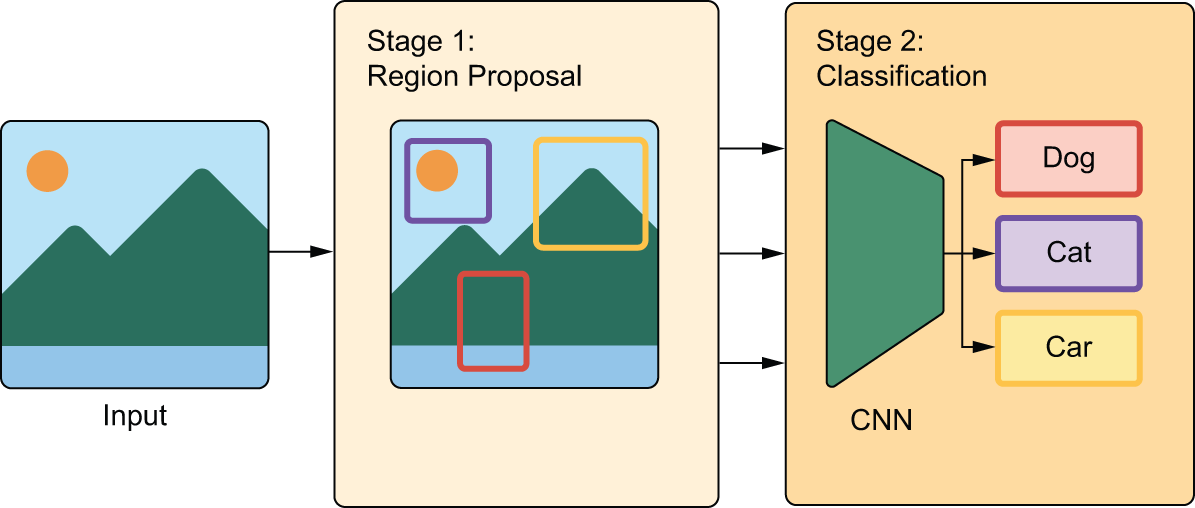
\includegraphics[width=\textwidth,height=0.6\textheight,keepaspectratio]{../../images/ch12/r-cnn-pipeline.8fe83666.png}
            \caption{Quy trình xử lý của R-CNN}
        \end{figure}
    \end{columns}
\end{frame}

\section{3. Kiến trúc Một giai đoạn (Single-stage Detectors)}

\begin{frame}{Kiến trúc Single-stage và FPN}
    \begin{columns}
        \column{0.5\textwidth}
        \begin{itemize}
            \item Dự đoán song song Tọa độ hộp và Nhãn ngay trong 1 bước duy nhất (YOLO, RetinaNet, SSD).
            \item \textbf{Vấn đề:} Vật thể nhỏ dễ bị mất dấu ở các lớp sâu.
            \item \textbf{Giải pháp FPN (Feature Pyramid Network):} Hợp nhất đặc trưng ở nhiều độ phân giải khác nhau, giúp mạng phát hiện được vật thể ở mọi kích cỡ (Từ nhỏ xíu đến to lớn).
        \end{itemize}
        
        \column{0.5\textwidth}
        \begin{figure}
            \centering
            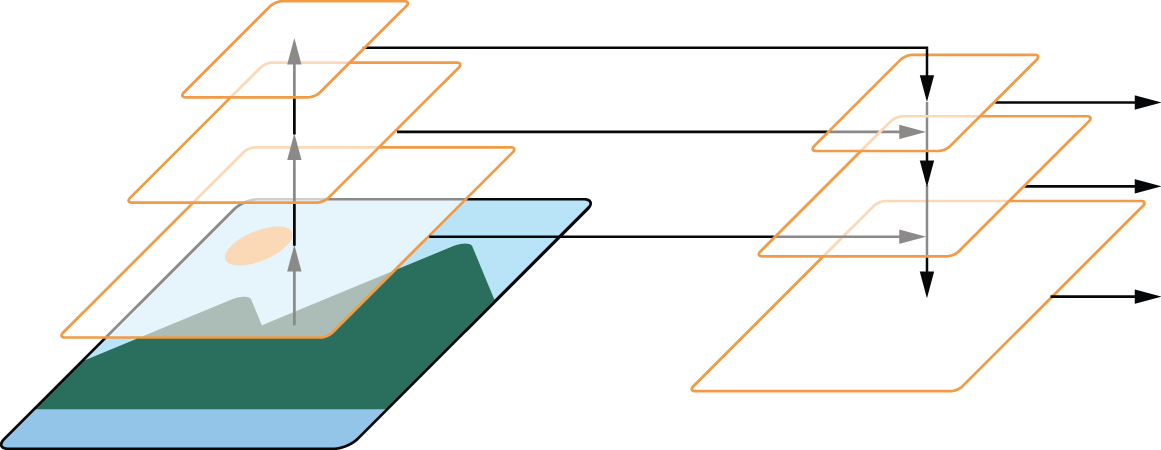
\includegraphics[width=\textwidth,height=0.6\textheight,keepaspectratio]{../../images/ch12/feature-pyramid-network.83b6f108.png}
            \caption{Mạng tháp đặc trưng (FPN)}
        \end{figure}
    \end{columns}
\end{frame}

\begin{frame}{Kết quả dự đoán của RetinaNet}
    \begin{columns}
        \column{0.5\textwidth}
        \begin{itemize}
            \item RetinaNet là một trong những Single-stage Detector xuất sắc nhất của Facebook AI.
            \item Sử dụng hàm \textbf{Focal Loss} để giải quyết bài toán mất cân bằng lớp trầm trọng giữa Tiền cảnh (Chứa vật thể) và Hậu cảnh (Không chứa gì).
            \item Dự đoán mượt mà, bao quát toàn bộ khung hình một cách chính xác.
        \end{itemize}
        
        \column{0.5\textwidth}
        \begin{figure}
            \centering
            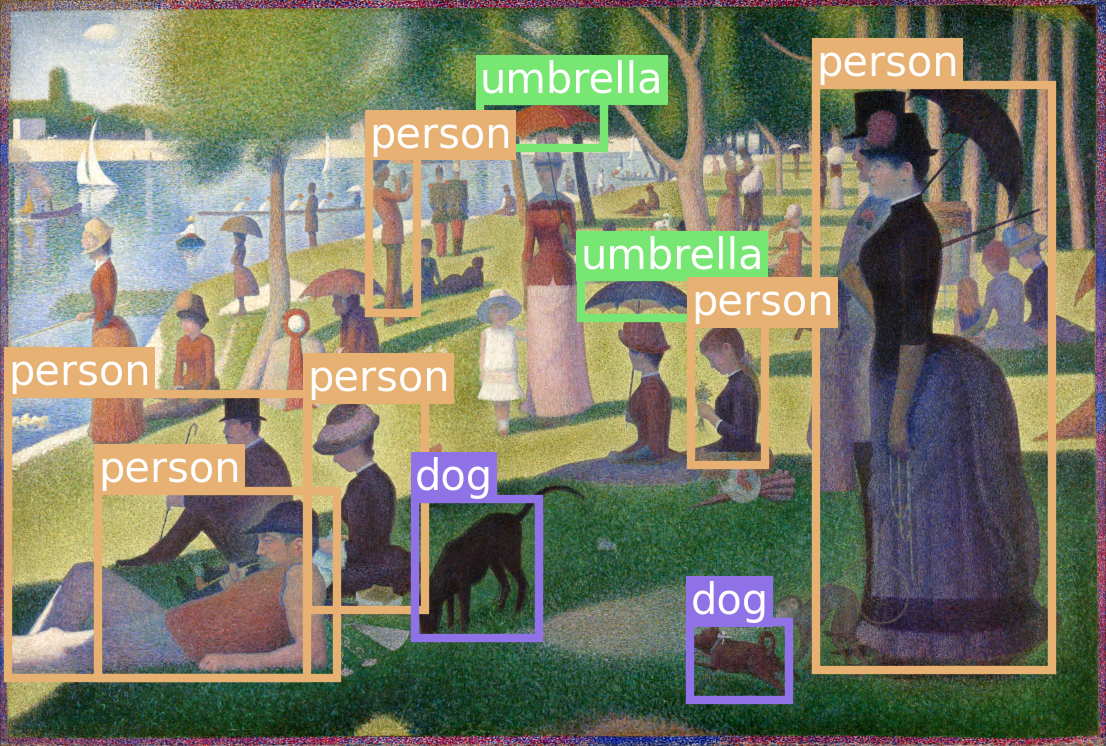
\includegraphics[width=\textwidth,height=0.6\textheight,keepaspectratio]{../../images/ch12/retinanet-output.0a67b6e8.png}
            \caption{Dự đoán của RetinaNet}
        \end{figure}
    \end{columns}
\end{frame}

\section{4. Thuật toán YOLO (You Only Look Once)}

\begin{frame}{Kỷ nguyên mới mang tên YOLO}
    \begin{itemize}
        \item Được giới thiệu năm 2015 bởi Joseph Redmon, YOLO làm rung chuyển giới AI.
        \item Chuyển bài toán Detection thành \textbf{Regression (Hồi quy) trên lưới (Grid)}.
        \item Khả năng chạy Real-time lên tới 45-155 FPS trên GPU, vượt xa hoàn toàn R-CNN.
        \item Nguyên lý: Chia ảnh thành lưới $S \times S$ (VD: $6 \times 6$). Mỗi ô lưới (Cell) chịu trách nhiệm dự đoán các vật thể có tâm (Center) nằm trong ô đó.
    \end{itemize}
\end{frame}

\begin{frame}{Tư duy Chia lưới và Anchor Boxes}
    \begin{columns}
        \column{0.5\textwidth}
        \begin{itemize}
            \item Hình bên trái: Chia ảnh gốc thành Lưới (Grid). Ô màu cam chứa Tâm của 1 con chó. Do đó ô lưới màu cam phải chịu trách nhiệm dự đoán con chó này.
            \item Hình bên phải: Mô hình sẽ không dự đoán tọa độ ngẫu nhiên. Nó sẽ xuất ra các đặc trưng Confidence, Bounding Box và Label cùng lúc.
        \end{itemize}
        
        \column{0.5\textwidth}
        \begin{figure}
            \centering
            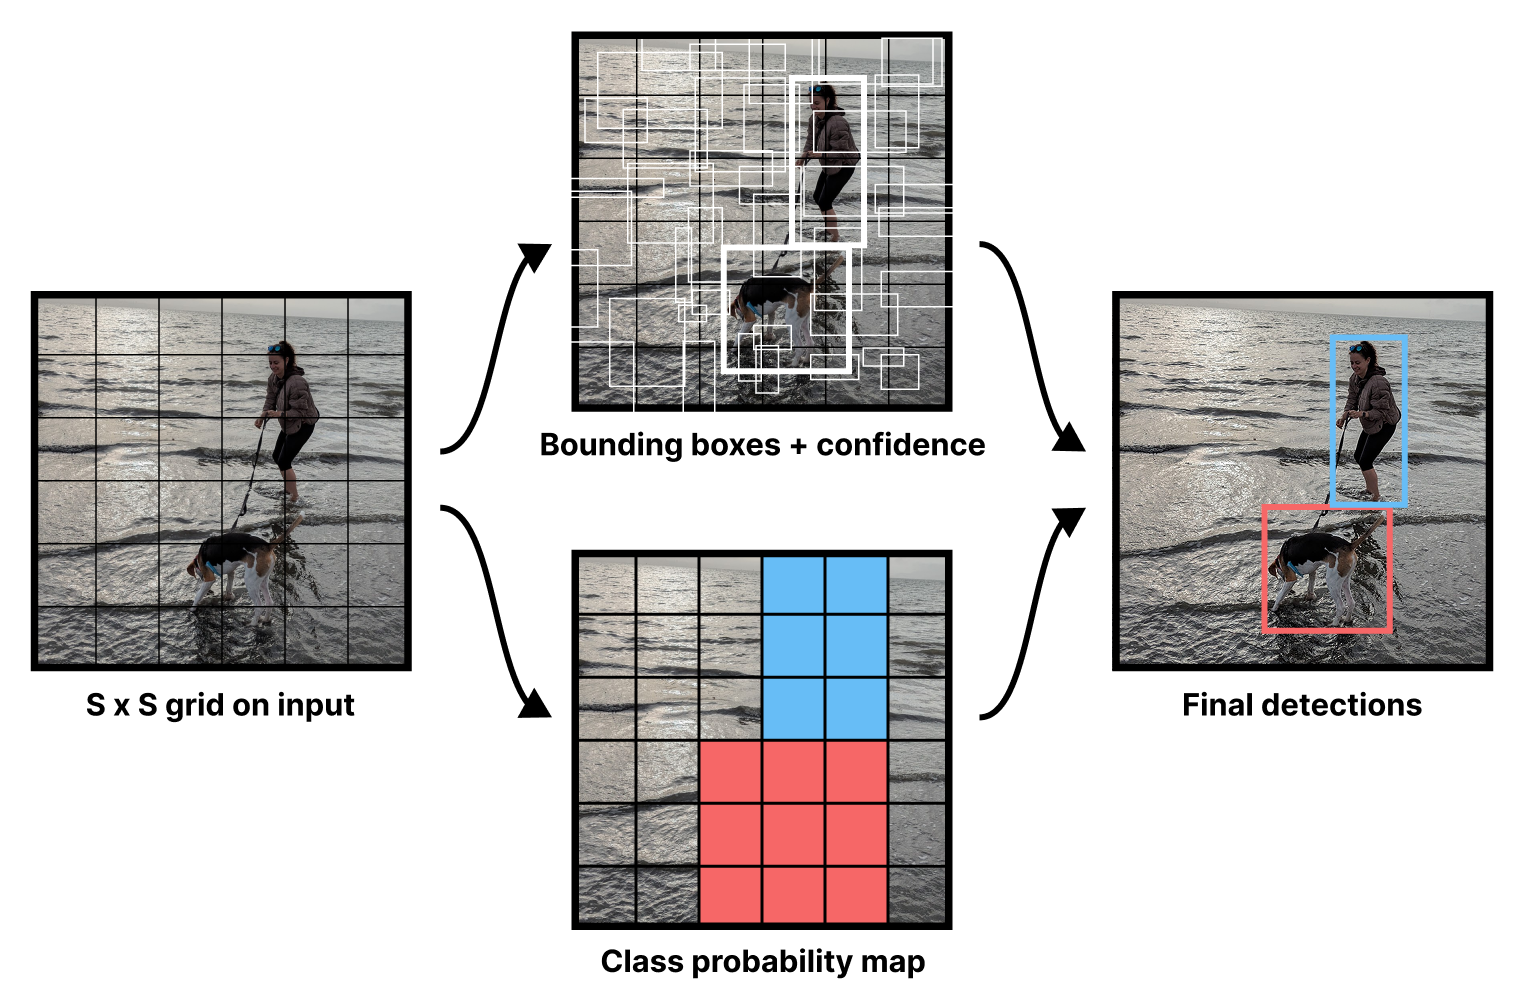
\includegraphics[width=\textwidth,height=0.5\textheight,keepaspectratio]{../../images/ch12/yolo-diagram.b7347ca6.png}
            \caption{Cơ chế hoạt động của YOLO}
        \end{figure}
    \end{columns}
\end{frame}

\begin{frame}[fragile]{Nạp Mạng Xương sống (Backbone)}
Thay vì đào tạo từ đầu, ta sử dụng mạng \texttt{ResNet50} đã được huấn luyện sẵn trên ImageNet từ \texttt{KerasHub} để đóng vai trò làm Bộ trích xuất Đặc trưng (Feature Extractor).

\begin{lstlisting}[language=Python]
image_size = 448

# Load ResNet50 pretrained backbone
backbone = keras_hub.models.Backbone.from_preset(
    "resnet_50_imagenet",
)

# Setup the preprocessor for input resizing
preprocessor = keras_hub.layers.ImageConverter.from_preset(
    "resnet_50_imagenet",
    image_size=(image_size, image_size),
)
\end{lstlisting}
\end{frame}

\begin{frame}[fragile]{Xây dựng Phần đầu YOLO (Prediction Head)}
Phần đặc trưng xuất ra từ ResNet sẽ được bóp phẳng và đưa qua 2 lớp \texttt{Dense} để biến thành thông tin Grid tọa độ.

\begin{lstlisting}[language=Python]
from keras import layers

grid_size = 6
num_labels = 91

inputs = keras.Input(shape=(image_size, image_size, 3))
x = backbone(inputs)
# Makes our backbone outputs smaller and then flattens the output
x = layers.Conv2D(512, (3, 3), strides=(2, 2))(x)
x = layers.Flatten()(x)

# Passes our flattened feature maps through densely connected layers
x = layers.Dense(2048, activation="relu", kernel_initializer="glorot_normal")(x)
x = layers.Dropout(0.5)(x)
x = layers.Dense(grid_size * grid_size * (num_labels + 5))(x)
\end{lstlisting}
\end{frame}

\begin{frame}[fragile]{Định hình Tensor Đầu ra}
Chuyển vector 1 chiều cuối cùng thành dạng Tensor $6 \times 6 \times (91 + 5)$. Sau đó cắt tách Box và Class riêng biệt.

\begin{lstlisting}[language=Python]
# Reshapes outputs to a 6 x 6 grid
x = layers.Reshape((grid_size, grid_size, num_labels + 5))(x)

# Split box and class predictions
# The first 5 values: x, y, w, h, confidence
box_predictions = x[..., :5]

# The next 91 values: Class probabilities using Softmax
class_predictions = layers.Activation("softmax")(x[..., 5:])

outputs = {"box": box_predictions, "class": class_predictions}
model = keras.Model(inputs, outputs)
\end{lstlisting}
\end{frame}

\begin{frame}[fragile]{Ánh xạ Tọa độ Hộp vào Lưới Grid}
Dữ liệu nhãn đang là kích thước toàn cục $([0,1])$. Cần chuyển hệ tọa độ tâm $(x,y)$ vào từng ô lưới nhỏ tương ứng.

\begin{lstlisting}[language=Python]
def to_grid(box):
    x, y, w, h = box
    cx, cy = (x + w / 2) * grid_size, (y + h / 2) * grid_size
    ix, iy = int(cx), int(cy)
    return (ix, iy), (cx - ix, cy - iy, w, h)

def from_grid(loc, box):
    (xi, yi), (x, y, w, h) = loc, box
    x = (xi + x) / grid_size - w / 2
    y = (yi + y) / grid_size - h / 2
    return (x, y, w, h)
\end{lstlisting}
\end{frame}

\begin{frame}[fragile]{Sinh Dữ liệu Lưới (Grid Targets)}
Vòng lặp ánh xạ hộp vào lưới. Mỗi ô lưới sẽ chứa thông tin về lớp đối tượng và hộp giới hạn (Chỉ gán nếu ô đó chứa vật).

\begin{lstlisting}[language=Python]
import numpy as np
import math

class_array = np.zeros((len(metadata), grid_size, grid_size))
box_array = np.zeros((len(metadata), grid_size, grid_size, 5))

for index, sample in enumerate(metadata):
    boxes, labels = sample["boxes"], sample["labels"]
    for box, label in zip(boxes, labels):
        # Transforms the box to the grid coordinate system
        (xi, yi), (grid_box) = to_grid(box)
        box_array[index, yi, xi] = [*grid_box, 1.0] # 1.0 is confidence
        
        # Makes sure the class label for the box's center location matches
        class_array[index, yi, xi] = label
\end{lstlisting}
\end{frame}

\begin{frame}{Toán học: Cấu trúc Vector Đầu ra}
    \begin{columns}
        \column{0.5\textwidth}
        Kết quả của đoạn Code vừa rồi tạo ra Vector gồm:
        \begin{enumerate}
            \item \textbf{$p_c$}: Confidence Score (Xác suất có chứa vật thể). Bằng $1.0$ nếu có vật.
            \item \textbf{$b_x, b_y$}: Tọa độ tâm của hộp giới hạn (Theo ô lưới).
            \item \textbf{$b_w, b_h$}: Chiều rộng, chiều cao của hộp (Toàn cục).
            \item \textbf{$c_1, c_2, ... c_k$}: Xác suất thuộc về class $i$ (Vd: Chó, Mèo, Xe).
        \end{enumerate}
        
        \column{0.5\textwidth}
        \begin{figure}
            \centering
            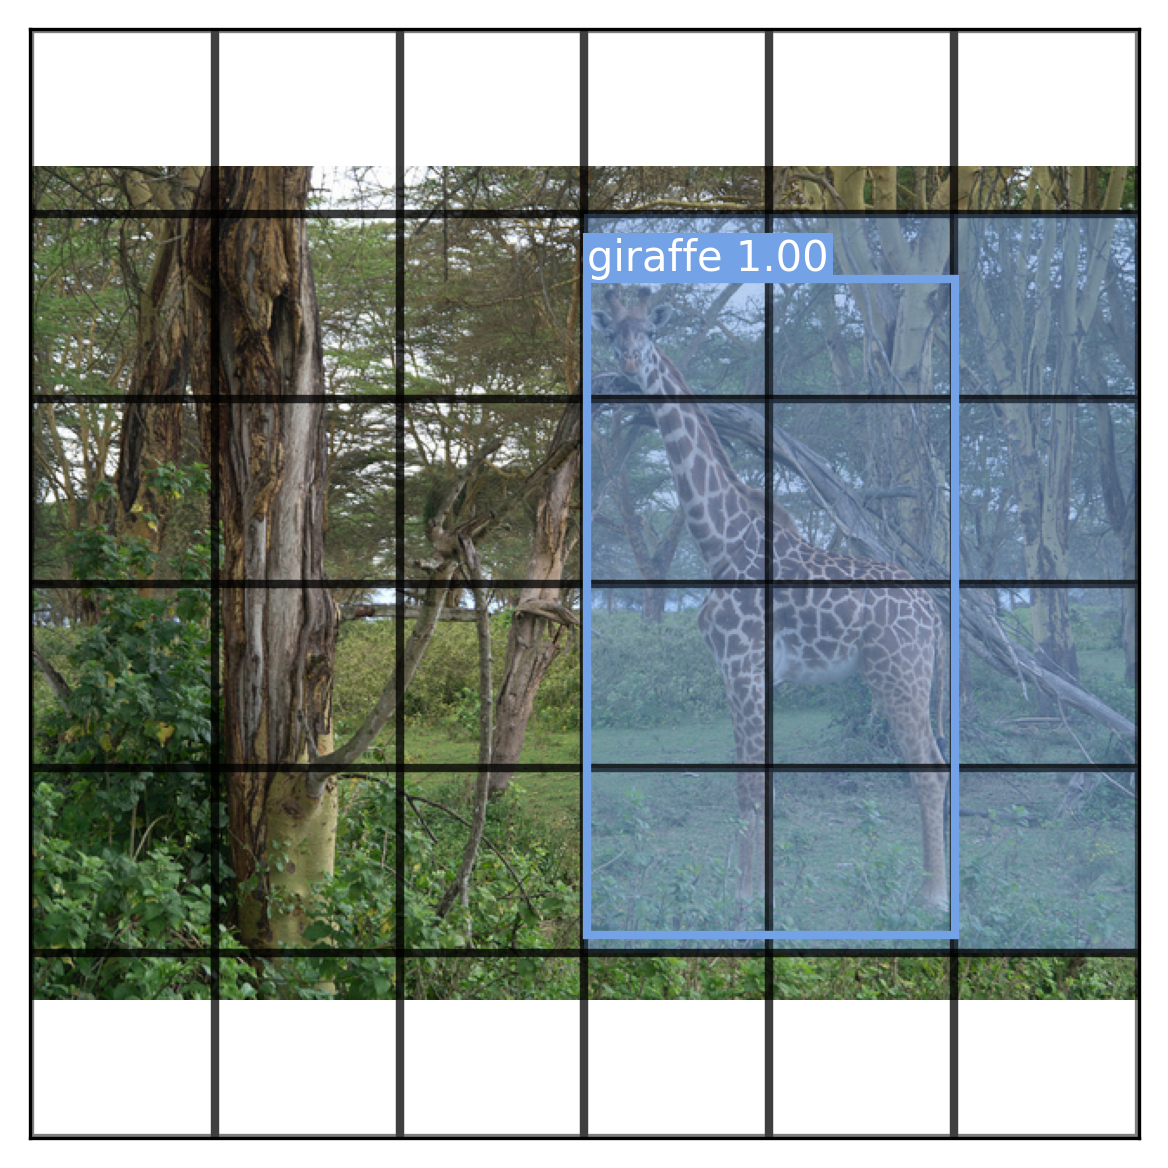
\includegraphics[width=\textwidth,height=0.6\textheight,keepaspectratio]{../../images/ch12/yolo-targets.7b3c7aed.png}
            \caption{Vector mục tiêu huấn luyện}
        \end{figure}
    \end{columns}
\end{frame}

\begin{frame}[fragile]{Sử dụng tf.data thiết lập Pipeline}
Tải ảnh song song (8 tiến trình), ghép nối Tensor mục tiêu và chia mẻ (Batch) kích thước 16. Sử dụng lệnh `prefetch` để chống thắt cổ chai GPU.

\begin{lstlisting}[language=Python]
import tensorflow as tf

def load_image(path):
    x = tf.io.read_file(path)
    x = tf.image.decode_jpeg(x, channels=3)
    return preprocessor(x)

images = tf.data.Dataset.from_tensor_slices([x["path"] for x in metadata])
images = images.map(load_image, num_parallel_calls=8)

labels = {"box": box_array, "class": class_array}
labels = tf.data.Dataset.from_tensor_slices(labels)

# Creates a merged dataset and batches it
dataset = tf.data.Dataset.zip(images, labels).batch(16).prefetch(2)
val_dataset, train_dataset = dataset.take(500), dataset.skip(500)
\end{lstlisting}
\end{frame}

\begin{frame}{Công cụ 1: Intersection over Union (IoU)}
    \begin{itemize}
        \item \textbf{IoU} là công thức toán học cốt lõi để tính toán độ trùng khớp giữa 2 Hộp giới hạn.
        \item IoU = (Diện tích phần Giao nhau) / (Diện tích phần Hợp nhau).
        $$ IoU = \frac{Area(Box_1 \cap Box_2)}{Area(Box_1 \cup Box_2)} $$
        \item IoU dao động từ $0$ (Không chạm nhau) đến $1$ (Trùng khớp hoàn toàn).
        \item Khác với Segmentation (IoU tính bằng Pixel), Detection (IoU tính bằng hình hộp chữ nhật).
    \end{itemize}
\end{frame}

\begin{frame}[fragile]{Viết hàm tính IoU trong Keras}
Chuyển lý thuyết thành Tensor operations để chạy song song trên GPU.

\begin{lstlisting}[language=Python]
from keras import ops

def unpack(box):
    return box[..., 0], box[..., 1], box[..., 2], box[..., 3]

def intersection(box1, box2):
    cx1, cy1, w1, h1 = unpack(box1)
    cx2, cy2, w2, h2 = unpack(box2)
    left = ops.maximum(cx1 - w1 / 2, cx2 - w2 / 2)
    bottom = ops.maximum(cy1 - h1 / 2, cy2 - h2 / 2)
    right = ops.minimum(cx1 + w1 / 2, cx2 + w2 / 2)
    top = ops.minimum(cy1 + h1 / 2, cy2 + h2 / 2)
    return ops.maximum(0.0, right - left) * ops.maximum(0.0, top - bottom)
\end{lstlisting}
\end{frame}

\begin{frame}[fragile]{Hàm Hợp nhau (Union)}
Tính tổng diện tích 2 hộp và trừ đi phần Giao, sau đó chia để tính tỷ lệ.

\begin{lstlisting}[language=Python]
def intersection_over_union(box1, box2):
    cx1, cy1, w1, h1 = unpack(box1)
    cx2, cy2, w2, h2 = unpack(box2)
    
    # Computes intersection
    intersection_area = intersection(box1, box2)
    
    # Computes union
    a1 = ops.maximum(w1, 0.0) * ops.maximum(h1, 0.0)
    a2 = ops.maximum(w2, 0.0) * ops.maximum(h2, 0.0)
    union_area = a1 + a2 - intersection_area
    
    # Divides gracefully, avoiding ZeroDivision
    return ops.divide_no_nan(intersection_area, union_area)
\end{lstlisting}
\end{frame}

\begin{frame}[fragile]{Định nghĩa Hàm Mất mát Hộp (YOLO Box Loss)}
Đây là tinh hoa của YOLO. Loss sẽ cộng dồn sai số tọa độ trung tâm, sai số căn bậc hai chiều cao/rộng, và sai số Confidence.

\begin{lstlisting}[language=Python]
def signed_sqrt(x):
    return ops.sign(x) * ops.sqrt(ops.absolute(x) + keras.config.epsilon())

def box_loss(true, pred):
    xy_true, wh_true, conf_true = true[..., :2], true[..., 2:4], true[..., 4:]
    xy_pred, wh_pred, conf_pred = pred[..., :2], pred[..., 2:4], pred[..., 4:]
    no_object = conf_true == 0.0
    
    xy_error = ops.square(xy_true - xy_pred)
    wh_error = ops.square(signed_sqrt(wh_true) - signed_sqrt(wh_pred))
    
    iou = intersection_over_union(true, pred)
    conf_target = ops.where(no_object, 0.0, ops.expand_dims(iou, -1))
    conf_error = ops.square(conf_target - conf_pred)
    # Continues on next slide...
\end{lstlisting}
\end{frame}

\begin{frame}[fragile]{Hệ số phạt (Penalty Scaling)}
Tác giả Redmon đề xuất tăng phạt x5 lần cho lỗi hộp và giảm nhẹ phạt x0.5 cho vùng không có đồ vật (Empty space).

\begin{lstlisting}[language=Python]
    # Concatenates the errors with scaling hacks
    error = ops.concatenate(
        (
            ops.where(no_object, 0.0, xy_error * 5.0),
            ops.where(no_object, 0.0, wh_error * 5.0),
            ops.where(no_object, conf_error * 0.5, conf_error),
        ),
        axis=-1,
    )
    # Returns one loss value per sample; Keras will sum over the batch.
    return ops.sum(error, axis=(1, 2, 3))
\end{lstlisting}
\end{frame}

\begin{frame}[fragile]{Huấn luyện Mô hình}
Cuối cùng, chúng ta đóng gói thành 1 quá trình biên dịch hoàn chỉnh. Loss của phân loại dùng hàm \texttt{sparse\_categorical\_crossentropy} chuẩn.

\begin{lstlisting}[language=Python]
# We use two separate loss functions for the two outputs
model.compile(
    optimizer=keras.optimizers.Adam(2e-4),
    loss={"box": box_loss, "class": "sparse_categorical_crossentropy"},
)

# Start training the detector
model.fit(
    train_dataset,
    validation_data=val_dataset,
    epochs=4,
)
\end{lstlisting}
Quá trình có thể tốn hàng giờ trên GPU do khối lượng tính toán quá khổng lồ.
\end{frame}

\begin{frame}{Kết quả Thô (Raw Predictions)}
    \begin{columns}
        \column{0.5\textwidth}
        \begin{itemize}
            \item Trong quá trình dự đoán (Inference), MỖI ô lưới sẽ xuất ra nhiều Bounding Boxes.
            \item Mô hình sinh ra \textbf{hàng trăm hộp giới hạn} cùng một lúc chồng chéo lên nhau.
            \item Hầu hết các hộp này là nhiễu, confidence rất thấp.
            \item Làm sao để dọn dẹp đống hỗn độn này?
        \end{itemize}
        
        \column{0.5\textwidth}
        \begin{figure}
            \centering
            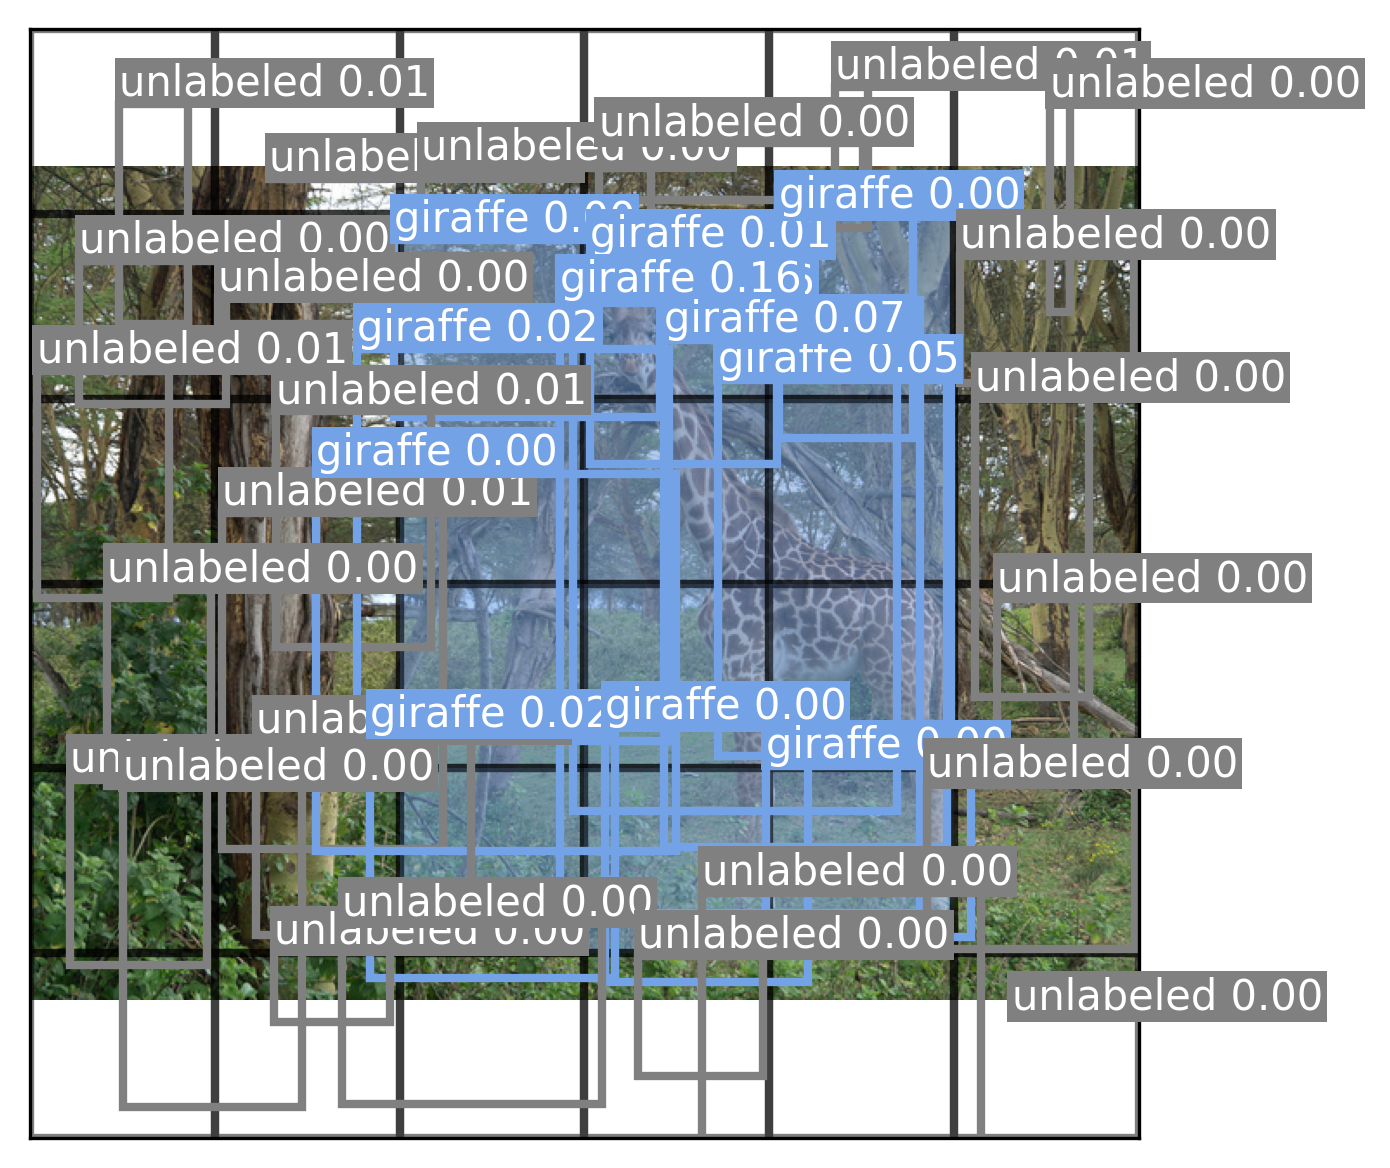
\includegraphics[width=\textwidth,height=0.6\textheight,keepaspectratio]{../../images/ch12/yolo-predictions-all.de18d520.png}
            \caption{Hàng ngàn hộp dự đoán thô}
        \end{figure}
    \end{columns}
\end{frame}

\begin{frame}{Công cụ 2: Non-Maximum Suppression (NMS)}
    Thuật toán NMS để lọc nhiễu hộp giới hạn:
    \begin{enumerate}
        \item Bỏ tất cả các hộp có Điểm tự tin (Confidence Score) quá thấp.
        \item \textbf{Vòng lặp:} Chọn hộp có Confidence Score \textbf{Cao nhất} làm chuẩn (Vd: Hộp chó $0.98$).
        \item Tính \textbf{IoU} của hộp chuẩn với tất cả các hộp Chó khác còn lại.
        \item Xóa toàn bộ các hộp có $IoU > 0.4$ (Vì chúng chắc chắn là bản sao trùng lặp của hộp chuẩn).
        \item Lặp lại đến khi không còn hộp nào chưa xét.
    \end{enumerate}
\end{frame}

\begin{frame}{Kết quả Cuối cùng (Sau khi chạy NMS)}
    \begin{columns}
        \column{0.5\textwidth}
        \begin{itemize}
            \item Sau khi trải qua bộ lọc Non-Maximum Suppression, từ hàng vạn hộp nhiễu, ta chỉ còn lại chính xác số lượng vật thể trong hình.
            \item YOLO vừa nhanh, vừa chính xác, thiết lập tiêu chuẩn công nghiệp (Industry Standard) cho mọi ứng dụng Camera AI, Flycam, và Xe tự lái hiện nay.
        \end{itemize}
        
        \column{0.5\textwidth}
        \begin{figure}
            \centering
            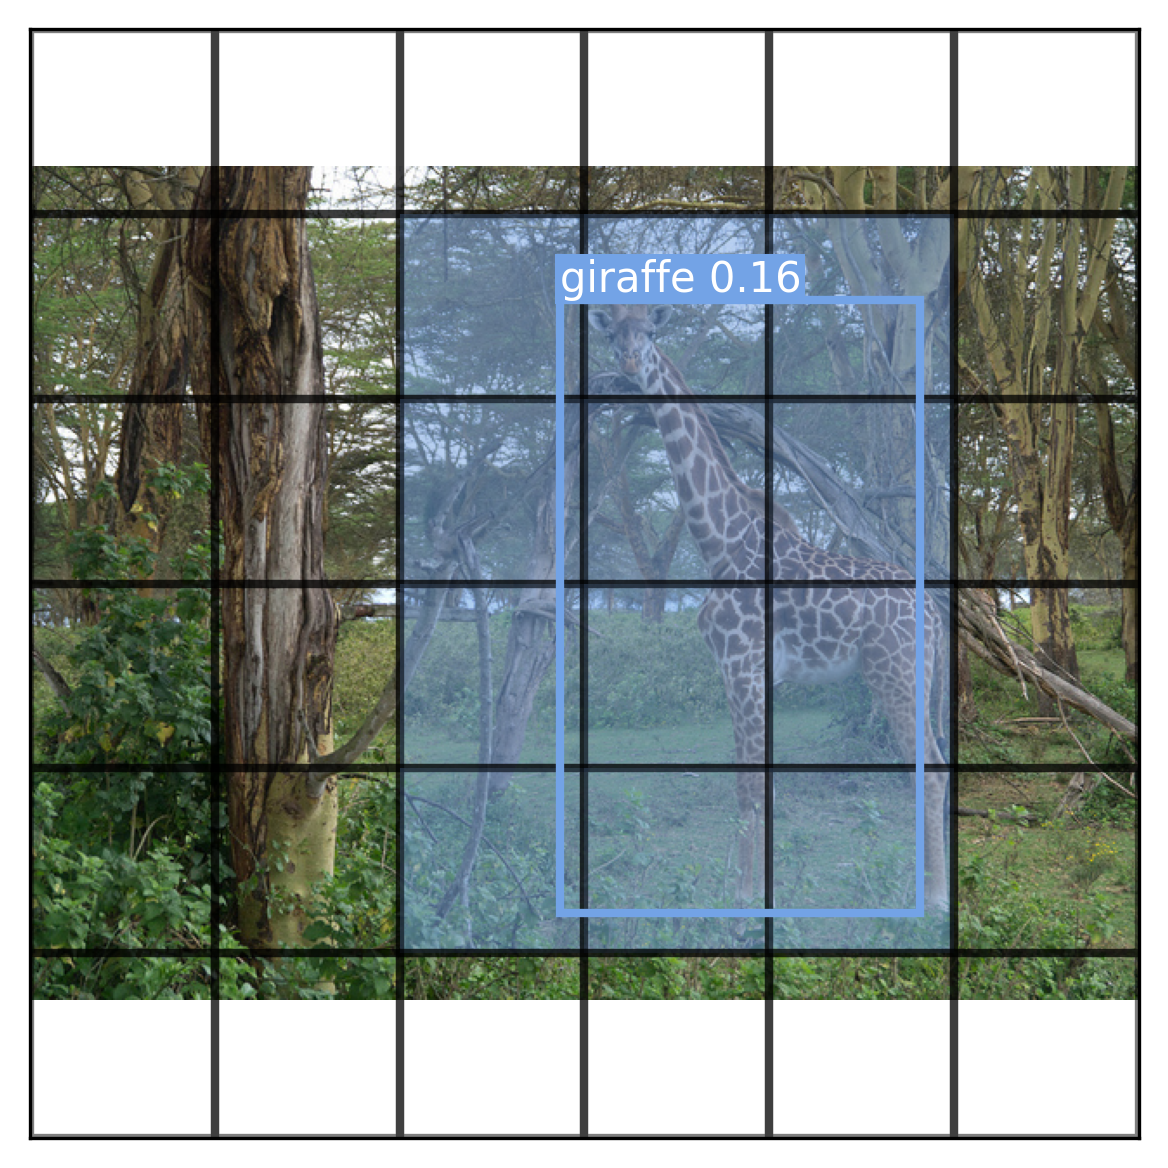
\includegraphics[width=\textwidth,height=0.6\textheight,keepaspectratio]{../../images/ch12/yolo-predictions.d621592d.png}
            \caption{Kết quả sạch sẽ sau NMS}
        \end{figure}
    \end{columns}
\end{frame}

\section{Tổng kết}

\begin{frame}{Tổng kết Chương 12}
    \begin{itemize}
        \item \textbf{Object Detection} phức tạp hơn Classification do phải giải quyết bài toán định vị (Localization).
        \item \textbf{Two-stage (R-CNN):} Quét vùng trước, Phân loại sau. Chậm nhưng chính xác.
        \item \textbf{Single-stage (YOLO, RetinaNet):} Gộp chung thành bài toán Hồi quy (Regression) trên lưới tọa độ. Nhanh và hiệu quả.
        \item Hiểu rõ các nguyên lý Toán học ẩn sau: Hồi quy Box $(x,y,w,h)$, đánh giá độ trùng khớp \textbf{IoU}, và thuật toán lọc nhiễu \textbf{NMS}.
    \end{itemize}
\end{frame}

\end{document}
